\documentclass[fontsize=8pt]{scrartcl}

% set document information
\title{ChipMulticoreProcessors}
\author{Fabian Olbert}                    % optional, delete if unchanged
% \myemail{info@latex4ei.de}           % optional, delete if unchanged
% \mywebsite{www.latex4ei.de}          % optional, delete if unchanged
% \usepackage{float}


\usepackage{amsmath}
\usepackage{xcolor}
% \usepackage{sectsty}
\usepackage{multicol}
\usepackage[a4paper, landscape, margin=0.5cm]{geometry}
\usepackage{microtype}
\usepackage{ulem}
\usepackage{listings}
\usepackage{graphicx}


\lstset{
  basicstyle=\ttfamily\footnotesize, % Smaller font for listings
  breaklines=true,                 % Allow lines to break
  captionpos=b,                    % Caption at the bottom
  numbers=left,                    % Line numbers on the left
  numberstyle=\tiny\color{gray},   % Style for line numbers
  showstringspaces=false           % Don't show spaces in strings with special char
}


% In your preamble
\definecolor{catBlue}{HTML}{0065bd}
\definecolor{nordicRed}{HTML}{FFFDE7	}

\makeatletter\let\inserttitle\@title\makeatother
\makeatletter\let\insertauthor\@author\makeatother

\usepackage{titlesec}

\titleformat{\section}[runin] % Command to customize
{\large\scshape\color{catBlue}} % Format for the whole heading (font, size, weight, color)
{\thesection  \quad} % The label (section number followed by a period)
{0.1cm } % Horizontal separation between label and title text
{} % Code to appear before the title text (e.g., \MakeUppercase)
[]

\titlespacing*{\section} % Use * version to affect first paragraph after heading too
{0pt} % Left margin (indentation of the heading itself)
{1.5ex plus 0.5ex minus 0.2ex} % Space BEFORE the heading (stretchable/shrinkable)
                                 % Default is often around 3.5ex plus 1ex minus .2ex
{0.5ex plus 0.2ex} % Space AFTER the heading (stretchable/shrinkable)
                     % Default is often around 2.3ex plus .2ex

\titleformat{\paragraph}[runin]
{\small\normalfont\scshape\ttfamily\color{black}}{}{0cm}{}

\titlespacing*{\paragraph}{0ex}{1.5ex}{3ex}

% custom commands:
\newcommand{\coloreq}[1]{\colorbox{nordicRed}{\(\displaystyle #1\)}}



% ======================================================================
% Begin
% ======================================================================
\begin{document}
\setlength{\columnseprule}{0.2pt}
\setlength{\parindent}{0pt}

\begin{multicols*}{4}

  \footnotesize


% ---- apply title
\noindent
{\Large\scshape\color{catBlue}\inserttitle} % Large, bold title
  %{\par\noindent\small\color{catBlue}\insertauthor} % Author name

\section{Overview}

\paragraph{moores's law} Transistors on a chip double every two years

\paragraph{Fixed versus Programmable Logic}

\begin{center}
  \centering
  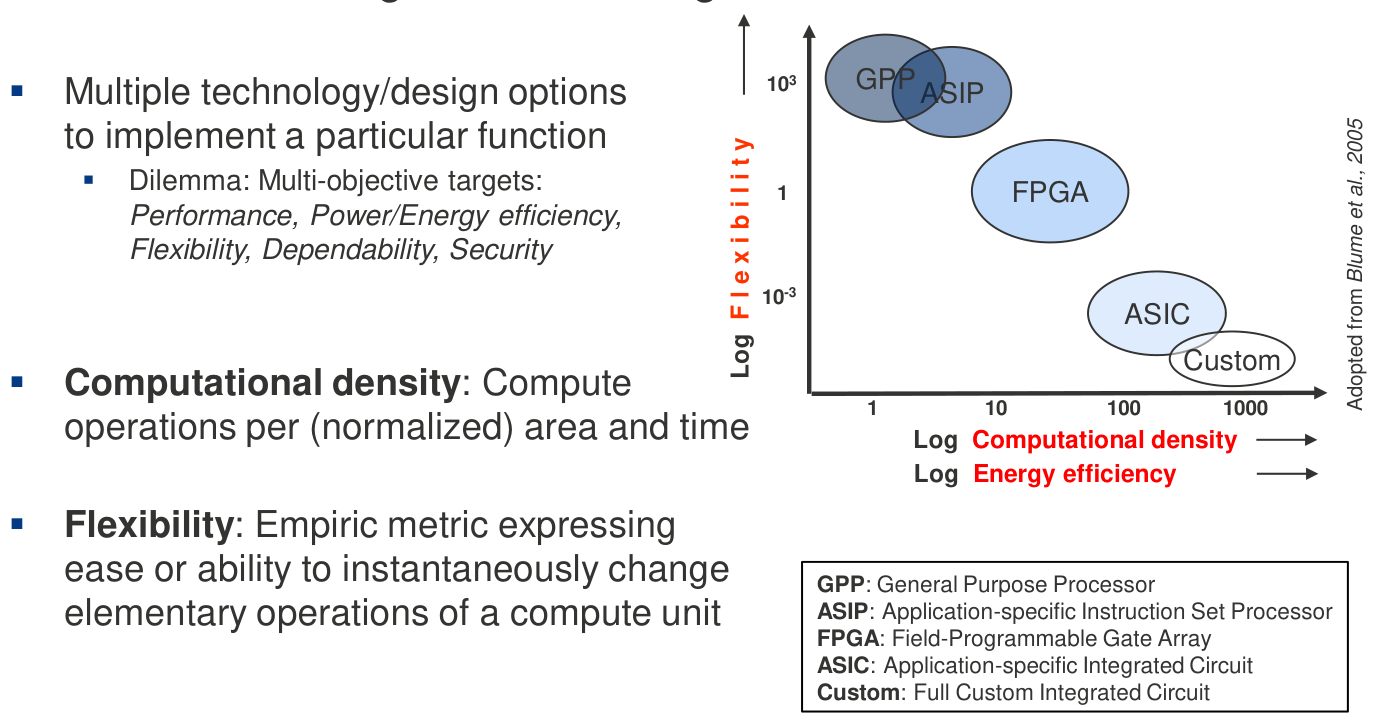
\includegraphics[width=0.8\linewidth]{img/FixedVsProgrammableLogic.png}
  \label{fig:fixedvsprogrammablelogic}
\end{center}

\paragraph{Evolution of Microarchitecture Improvements}

\begin{center}
  \centering
  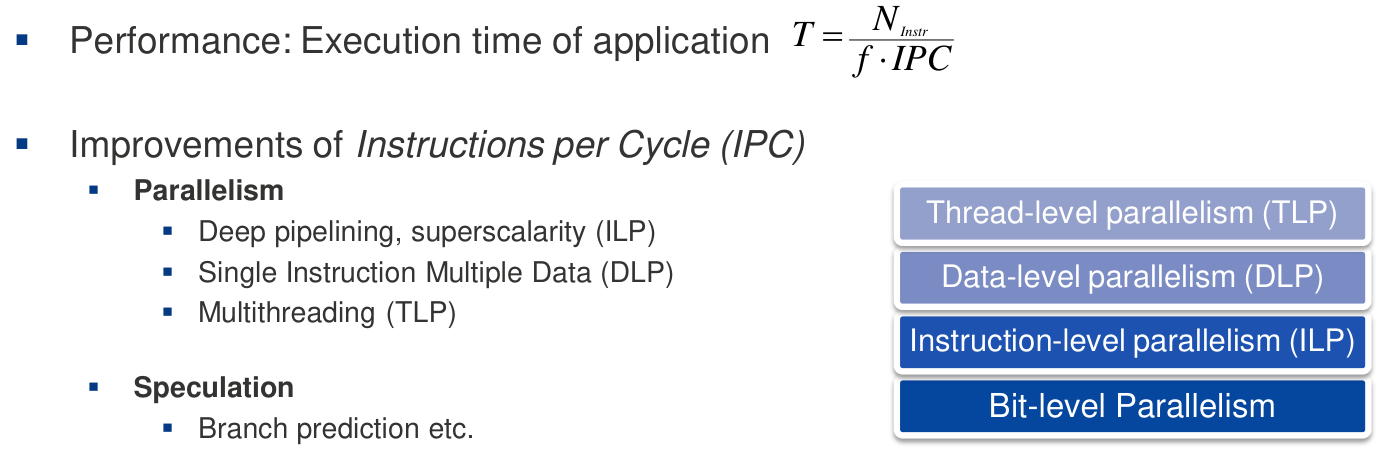
\includegraphics[width=0.8\linewidth]{img/EvolutionMicroarchitecture.png}
  \label{fig:evolutionmicroarchitecture}
\end{center}

\paragraph{ILP and DLP}

\begin{center}
  \centering
  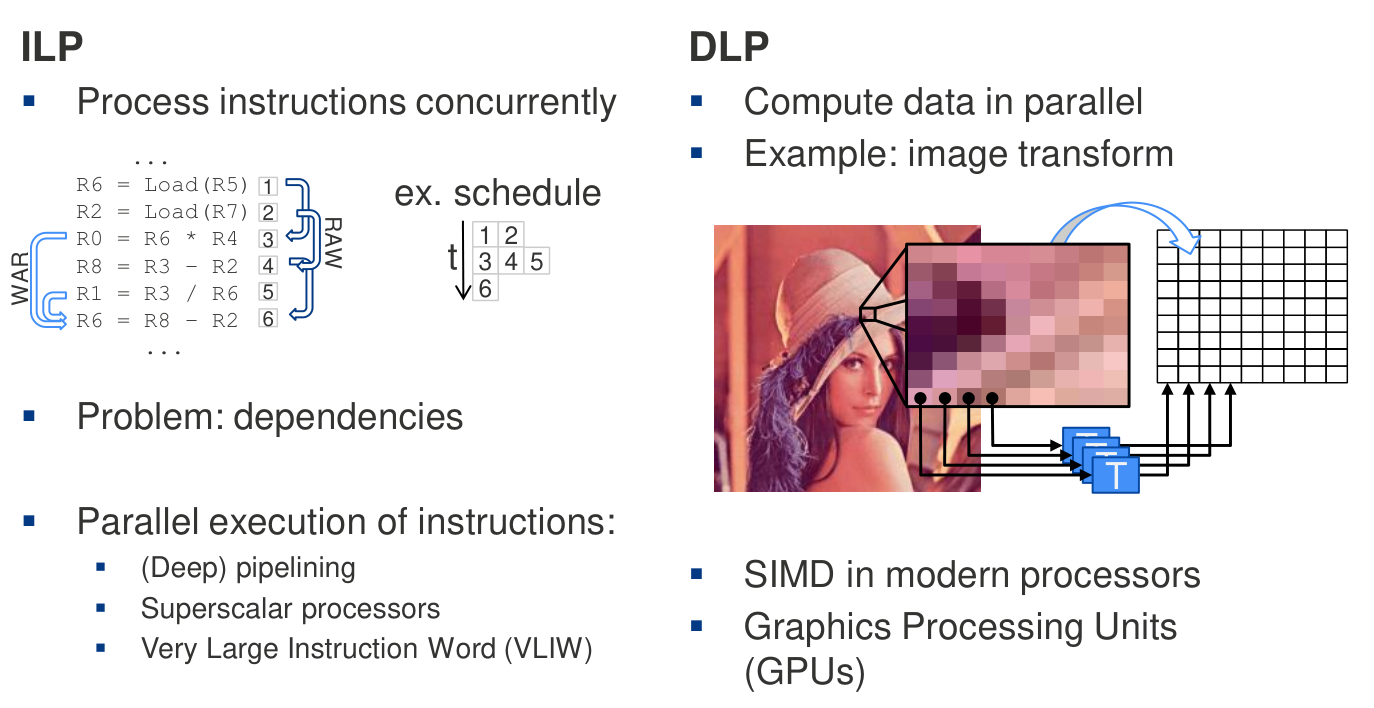
\includegraphics[width=0.8\linewidth]{img/ILPDLP.png}
  \label{fig:ilpdlp}
\end{center}

\begin{center}
  \centering
  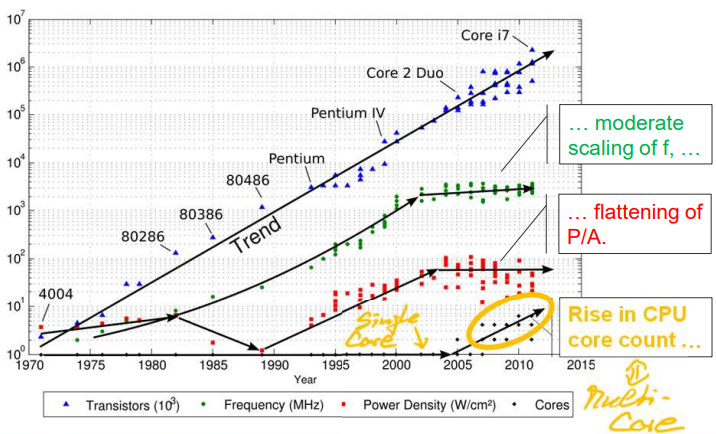
\includegraphics[width=\linewidth]{img/power_wall.png}
  \label{fig:power_wall}
\end{center}

\paragraph{Thread Level Parallelism}

\begin{center}
  \centering
  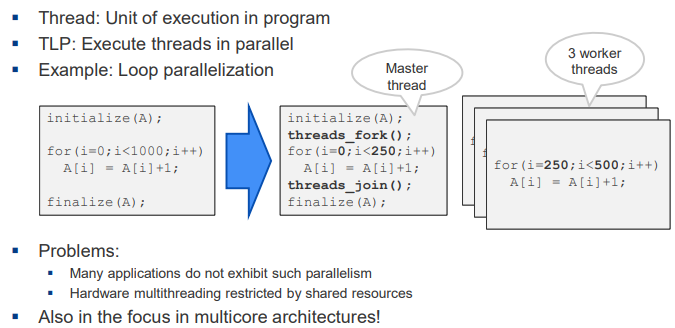
\includegraphics[width=0.8\linewidth]{img/TLP.png}
  \label{fig:tlp}
\end{center}

\paragraph{from microarchitecture to macroarchitecture}

\begin{center}
  \centering
  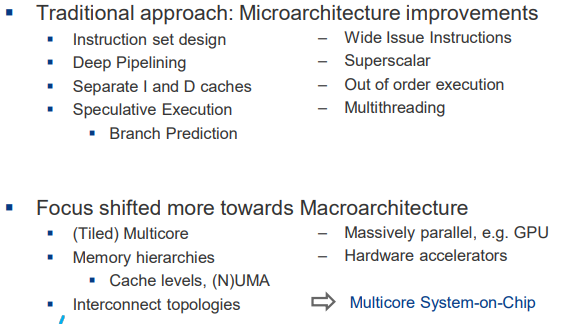
\includegraphics[width=0.8\linewidth]{img/frommicrotomacro.png}
  \label{fig:frommicrotomacro}
\end{center}

\paragraph{dynamic power dissipation} \coloreq{{P_{dyn} = \alpha C f V_{dd}^2 \cdot N_{core}}}

\paragraph{processor coefficient} \coloreq{\delta_0 = \alpha \cdot C}

\paragraph{power density} \coloreq{ Pd = \frac{P_{dyn}}{area \cdot N_{cores}} \quad [\frac{W}{cm^2}]}

\paragraph{instructions per second} \mbox{} \\ 
\indent \coloreq{ IPS = IPC \cdot f_{clk} \quad [\text{MIPS or GIPS}]}

\paragraph{propagation delay} \coloreq{t_{pd} \sim C \cdot \frac{1}{V_{dd} - V_t}} 

\paragraph{calculte new voltage} \coloreq{t_{pd,1} = N_{cores} \cdot t_{pd,N}}

\coloreq{\hat{V_{dd}} = \frac{V_{dd} + (N_{core} - 1) V_{th}}{N_{core}}}

\paragraph{amdahl's law} parallel execution time: \newline 
\indent\coloreq{T' = (s + \frac{p}{N_p}) T}

\coloreq{T = \frac{N_{instr}}{f \cdot IPC}}

\paragraph{speedup} \coloreq{\frac{T}{T'} = \frac{1}{s + \frac{p}{N}}}

\paragraph{utilization} calculate the utilization of each core and use the average in the end 

\coloreq{c_{sequenctial,core} = 1} 

\coloreq{c_{parallel,core} = \frac{\#parallelCycles}{\#totalCycles}}

\paragraph{frequency} \coloreq{f = \frac{IPS}{IPC} \cdot (s + \frac{p}{N})}




\section{Synchronization}

% \paragraph{Critical Sections}...

\paragraph{Mutual Exclusion}Only one thread enters critical section
, Wait while other thread in critical section

\begin{lstlisting}[language=c, numbers=none]
pthread_mutex_t;
pthread_mutex_lock(&lock);
pthread_mutex_unlock(&lock);

while (tmp == 0){
pthread_mutex_unlock(&lock); \\ no deadlock
pthread_mutex_lock(&lock);
}
\end{lstlisting}

\paragraph{Basic Lock Propertis}
  \begin{enumerate}
    \item Mutual exclusion
    \item Deadlock-freedom (liveness)
    \item Starvation-freedom
  \end{enumerate}

\paragraph{Atomicity}Each critical section appears atomic (indivisible) to other threads, Leads to linearization of accesses:

\paragraph{Spinlocks vs. Blocking}“Busy waiting” vs supending(), efficient for short critical sections vs long, no context switch vs context switch

\paragraph{Semaphore}...

\paragraph{Monitors}...

\paragraph{Signaling and Waiting}...

\paragraph{Condition Variables}
allows processor to do sth else and be notified instead of busy waiting, what makes it less cpu hungry (is slower than waiting because of context switch)
\begin{enumerate}
  \item[$\bullet$] \texttt{wait()}: append thread to queue of waiting threads, suspend thread
  \item[$\bullet$] \texttt{signal()}: pop thread from queue, reactivate thread
  \item[$\bullet$] \texttt{broadcast()}: reactivate all threads in queue
\end{enumerate}   

\begin{lstlisting}[language=c, numbers=none]
pthread_cond_t cond;
void write(int write_value);
pthread_mutex_lock(&lock) // before critical section
while (tmp == STACK_SIZE){
pthread_cond_wait(&cond, &mutex);} // instead of double mutex
//critical section
pthread_cond_signal(&cond)
pthread_mutex_unlock(&lock) // after critical section
\end{lstlisting} %s

\paragraph{Peterson Lock} software solution for 2 threads

\paragraph{multi thread solution} filter lock or baker's lock 

\paragraph{Barriers}...

\paragraph{Coarse-grained Locking} ...

\paragraph{Fine-grained Locking} a

\begin{center}
  \centering
  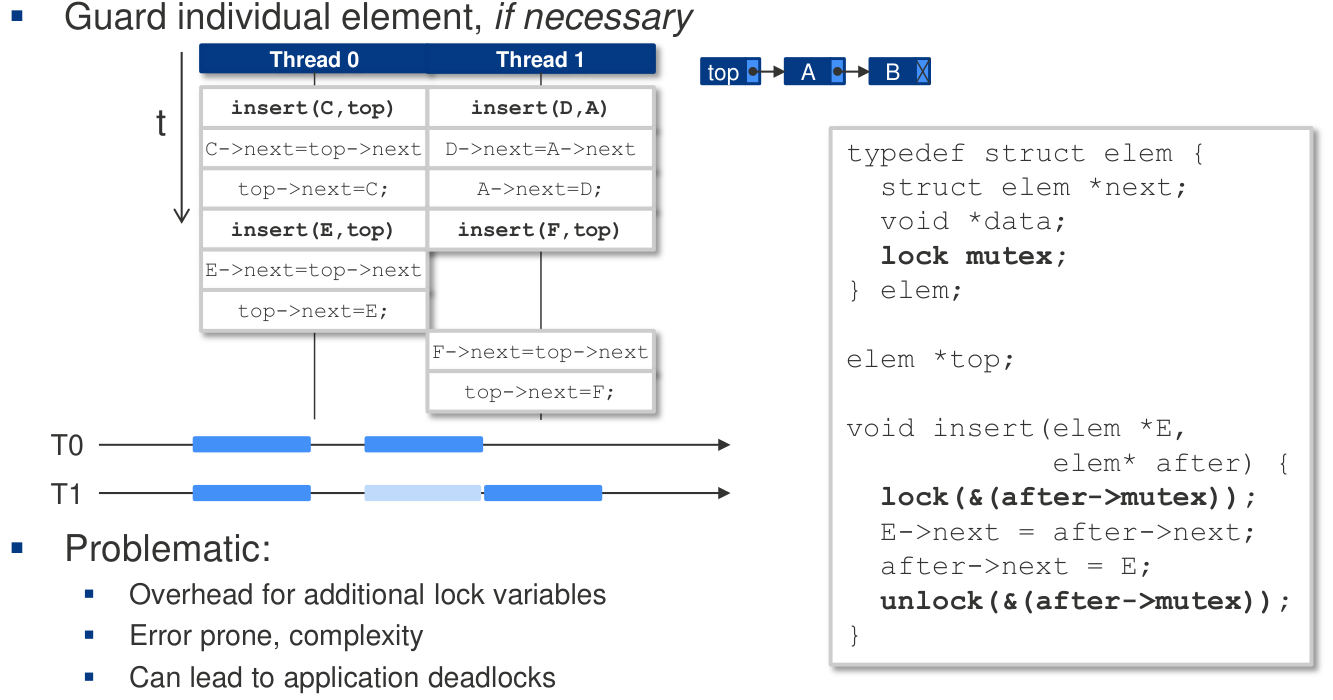
\includegraphics[width=0.8\linewidth]{img/fineGrainedLock.png}
  \label{fig:finegrainedlock}
\end{center}

\paragraph{CMP Tutorial – Performance of NBDS vs. Locks}

\begin{center}
  \centering
  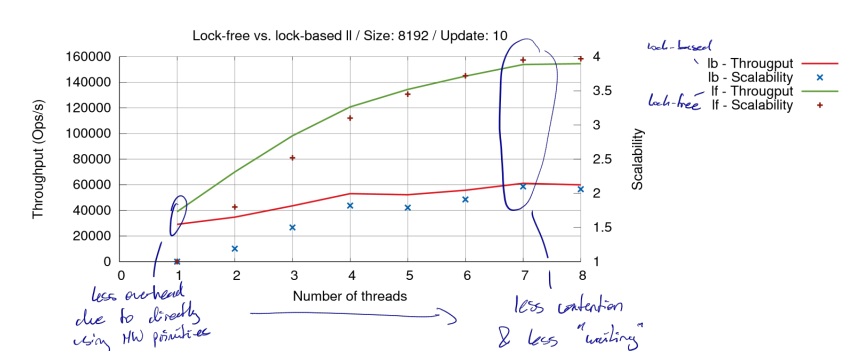
\includegraphics[width=\linewidth]{img/NBDSVsLocks.png}
  \label{fig:nbdsvslocks}
\end{center}

\paragraph{Compare-and-swap} read value, if value matches compare value: swap, if it does not match: leave old value, return value  - only operates on one word, aba problem

\begin{center}
  \centering
  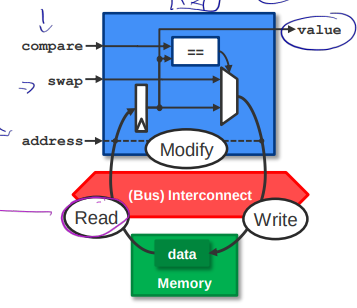
\includegraphics[width=0.4\linewidth]{img/compareAndSwap.png}
  \label{fig:compareandswap}
\end{center}

\begin{lstlisting}[language=c, numbers=none]
  int cas(int* addr, int compare, int swap) {
    int tmp=*addr;
    if (tmp==compare) {
      *addr=swap;
    }
    return tmp;
  } 
\end{lstlisting} %s

\begin{lstlisting}[language=c, numbers=none]
  void push(elem *E) {
    elem *tmp;
    do {
      tmp=top->next;
      E->next=tmp;
    } while (CAS(&top->next,tmp,E)!= tmp);
  }
\end{lstlisting} %s

\paragraph{ABA problem}A concurrency issue where a memory location's value changes from A \(\to\) B \(\to\) A between a read and a CAS attempt. The CAS operation, only seeing 'A' again, falsely assumes no modification occurred, even though the value was updated., only happens with CAS, not LL/SC


\paragraph{Load-Linked(LL)/Store-Conditional(SC)} \mbox{}
\begin{multicols*}{1}Load-link returns the current value of a memory location, while a subsequent store-conditional to the same memory location will store a new value only if no updates have occurred to that location since the load-link.


\begin{center}
  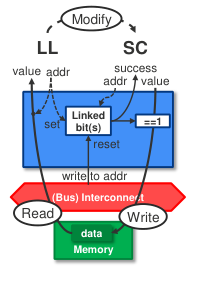
\includegraphics[width=\linewidth]{img/load-linked_overview.png}
  \label{fig:load-linked_overview}
\end{center}
\end{multicols*}

pseudocode:

\begin{lstlisting}[language=c, numbers=none]
  int linked[] = { 0 };
  int ll(int *addr){
    linked[addr] = 1;
    return *addr;
  }

  void on_anymem_write_access(int *addr){
    linked[addr] = 0;
  }

  bool sc(int *addr, int value) {
    if (linked[addr] == 1) {
      *addr = value;
      linked[addr] = 0;
      return true;
    }
    return false;
  }
\end{lstlisting} %s

usage stack:

\begin{lstlisting}[language=c, numbers=none]
  elem* pop() {
    elem *ret,*nxt;
    do {
      ret=LL(top->next);
      nxt=ret->next;
    } while (!SC(&top->next,nxt));
    return ret;
  }
\end{lstlisting} %s



\paragraph{Problem Set of Synchronization Primitives}...

\begin{center}
  \centering
  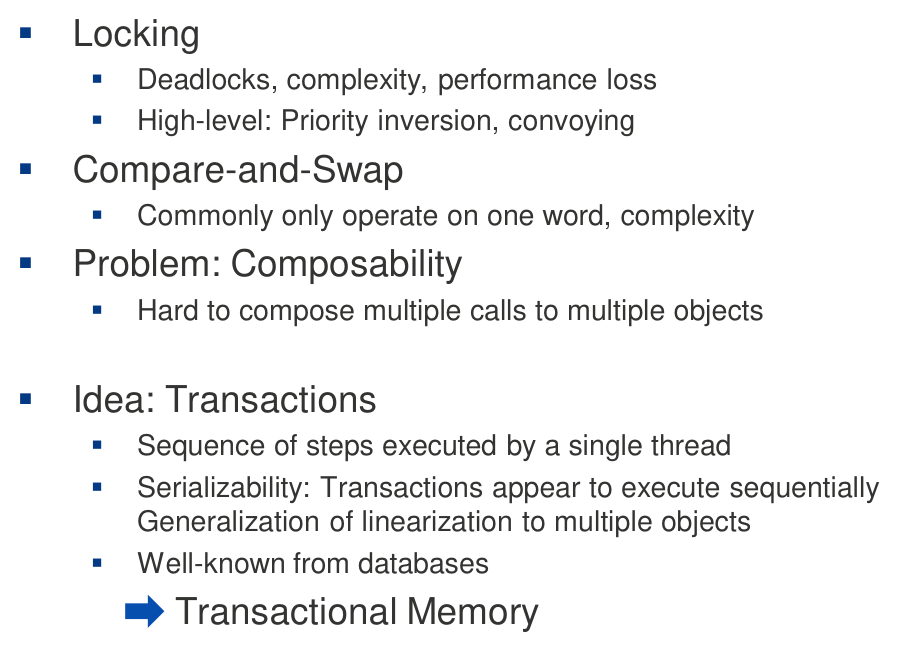
\includegraphics[width=0.8\linewidth]{img/problemSynchrPrimitives.png}
  \label{fig:problemsynchrprimitives}
\end{center}

\paragraph{Transactional Memory} Define sequence of instructions as an atomic block. - performance issues with big blocks

\paragraph{Software Transactional Memory}

\begin{center}
  \centering
  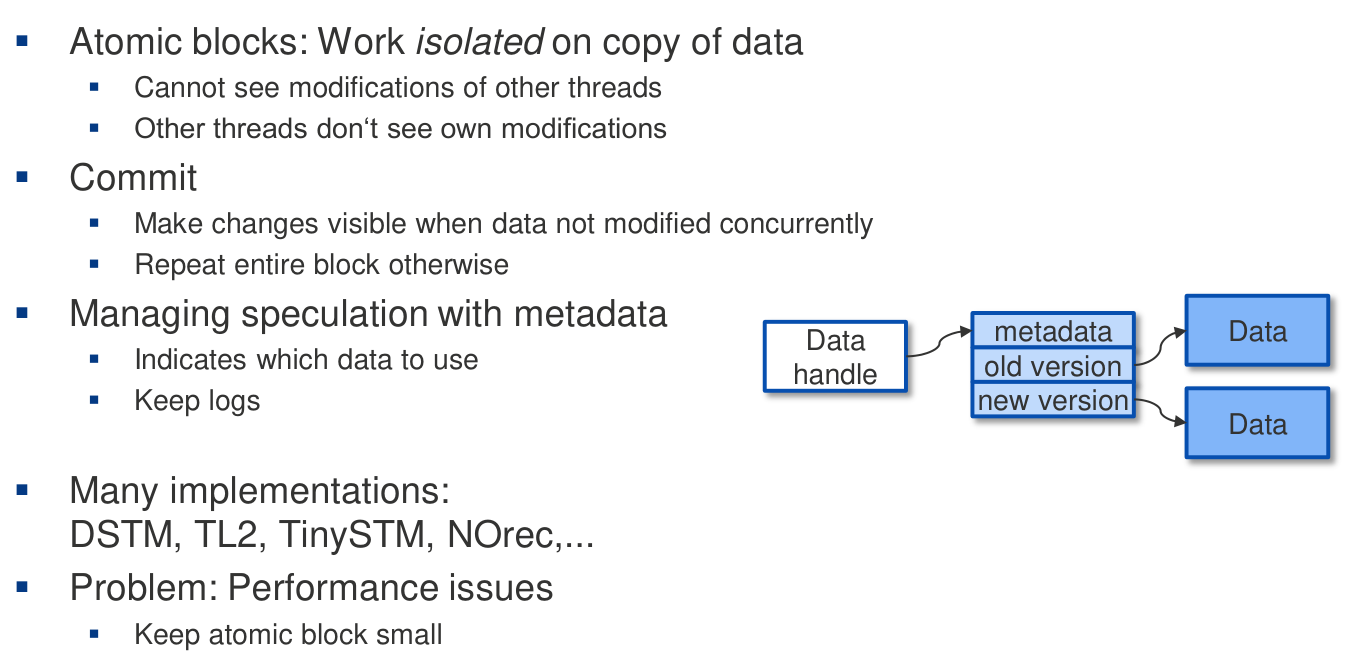
\includegraphics[width=0.8\linewidth]{img/SoftwareTransMemory.png}
  \label{fig:softwaretransmemory}
\end{center}

\begin{lstlisting}[language=c, numbers=none]
void insert(elem *E, elem* after) {
  atomic {
    E->next = after->next;
    after->next = E;
  }
}

void remove(elem *E) {
  atomic {
    elem *prev=get_prev(E);
    prev->next=E->next;
  }
}
\end{lstlisting} %s

\paragraph{CMP Tutorial – Synchronization Recap}

\begin{center}
  \centering
  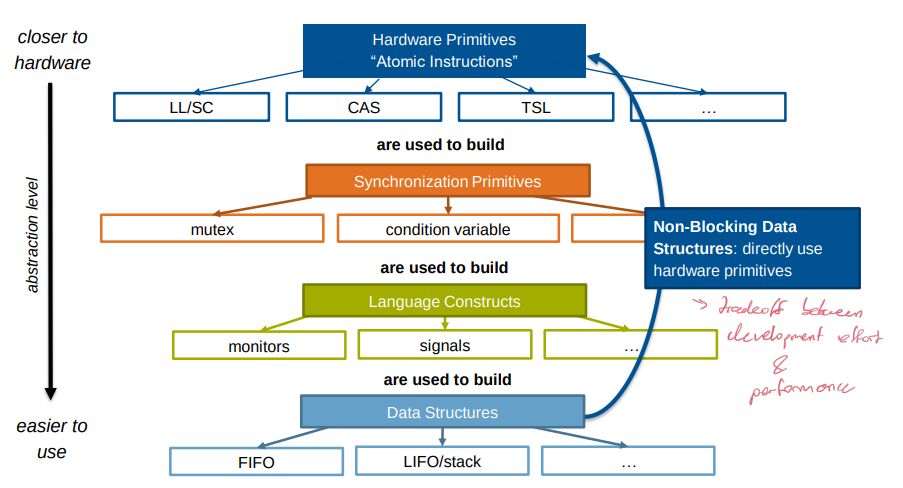
\includegraphics[width=0.8\linewidth]{img/SynchronizationRecap.png}
  \label{fig:synchronizationrecap}
\end{center}


\section{Memory}

\paragraph{Memory Wall} Access latencies of (DRAM) memoreis did not improve the same way as Processors did. This leads to a gap between the invrease of CPU and memory performance of around 30\% per year.

\begin{center}
  \centering
  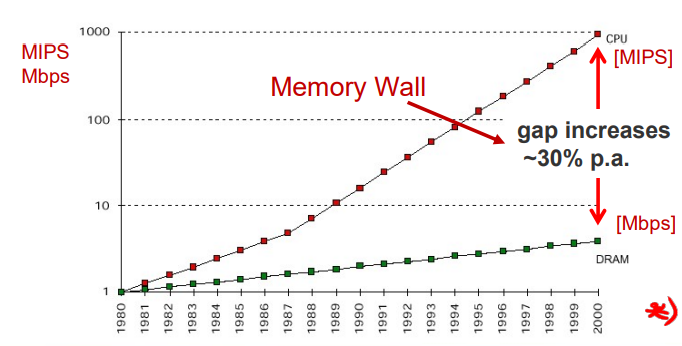
\includegraphics[width=0.8\linewidth]{img/memoryWall.png}
  \label{fig:memorywall}
\end{center}

\paragraph{Performance of Memory Subsystem without Cache} 

\coloreq{CPI_{mem} = CPI_{mem,instr} + CPI_{mem,d}} \\

\noindent
If the instructions are located in memory, the processor has to retrieve the instructions from memory and has to access memory for every instructions that accesses data.

\coloreq{r_{acc} = r_{acc,inst} + r_{acc,data}}

where $r_{acc}$ is the rate at which data is accessed


\paragraph{Performance of Memory Subsystem with Cache} 
$CPI = CPI_{cpu} + CPI_{mem}$ \\
$CPI_{mem} = r_{acc}((T_{cache} \cdot f_{cpu}) + r_{miss} \cdot T_{DRAM} \cdot f_{cpu})$ \\
\coloreq{CPI_{mem} = r_{acc}(CPI_{cache}) + r_{miss} \cdot CPI_{DRAM})}

\coloreq{r_{acc,local} = \frac{r_{acc,global}}{r_{acc, local, prev}}}

\paragraph{Memory Hierarchy} Up to 3 levels: L1, L2, L3. Performance/cost optimization: fast small caches nearer to the core, bigger caches with higher associativity (increased hit rate but higher latency) and thus lower miss rate far from core. L1 cache is part of the core.

\paragraph{Cache Organization}
\begin{center}
  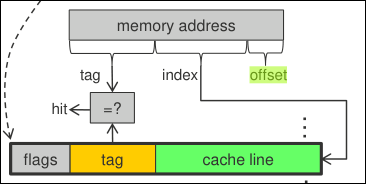
\includegraphics[width=0.8\linewidth]{img/CacheLine.png}
  \label{fig:cacheline}
\end{center}

\textit{Index:} used to determine potential position(s) in cache

\textit{Tag:} part of address stored together with cache line. If stored tag is identical to tag part of memory address+ flag = valid Cache hit

\textit{Offset:} determines word in cache line and byte in word

\coloreq{Nbit_{offset} = log_2(Bytes Cache Line)}

\coloreq{Nbit_{index} = log_2(NSets)}

\coloreq{Nbit_{tag} = Bits_{Address} - Bits_{Offset} - Bits_{Index}}

\paragraph{Direct Mapped Cache} Each block (size of a cache line) in mainmemory can be stored in only one cache entry. Direct mapped chaches are fast; L1 caches, but higher miss rate.

\paragraph{Set Associative Cache} Each block in main memory can be storedin n cache entries: n-way set associative cache Increasing n reduces cache misses due to conflicts.

\paragraph{Fully Associative Cache}A memory block can be stored in any cache entry. Only one set containing all entries. No cache misses due to conflicts

\paragraph{Temporal locality} A data item accessed once is a good candidate to be accessed again. For example loop instructions.

\paragraph{Spatial locality} Surrounding data in the same cache line is potentially accessed in the following. For example in data (arrays).

\paragraph{Cache Replacement} necessary on cache miss when all associated entries occupied: replace one entry.
Direct mapped cache: replace old entry with new.
Fully associative cache: replace only when full.
Set associative cache: choose replacement policy.

\paragraph{Cache Replacement Policy}
Goal: reduce number of misses

Least recently used (LRU): least recently access

First in first out (FIFO): least recently loaded (oldest)

Random

\paragraph{Cache Write Strategies} 
write-back: Modified data written directly through, Drawback: High traffic load at memory controller

write-through: Modify data locally, dirty flag marks updated chache line, dirty cache lines are written back on: replacement, by invalidation or by cache coherence protocol

\paragraph{Cache Misses}
\begin{enumerate}
  \item[$\bullet$] \textit{Compulsory} When Data is first loaded - can't be avoided
  \item[$\bullet$] \textit{Capacity} When cache is to small - larger cache
  \item[$\bullet$] \textit{Conflict} when data was previously replaced - higher associaty
\end{enumerate}

\noindent
$CPI_{mem} = r_{acc} \cdot f_{cpu}(r_{miss1} \cdot (T_{C2} + r_{miss2} \cdot (T_{C3} + r_{miss3} \cdot T_{DRAM})))$

\paragraph{in Real time systems} Caches are often not used since the caches only improve the average memory access latency and not the worst case execution time.

\paragraph{SDRAM Read Access Operation} \mbox{}   %s 

\noindent
Bandwidth metrics:

\noindent
$BW_{peak} = f_{mem} \cdot w$

\noindent
$BW_{burst,n} = 
\begin{cases}
\frac{f_{\text{mem}} \cdot w \cdot n}{t_{RC}} & , n \leq t_{RC} - t_{\text{mem\_acc}} \\[2ex]
    \frac{f_{\text{mem}} \cdot w \cdot n}{t_{\text{mem\_acc}} + (n-1)} & , \text{else}
\end{cases}$
$BW_{single word} = \frac{f_{mem} \cdot w}{t_{RC}}$

\noindent
Latency metrics:

\noindent

$t_{memAcc} = t_{RCD} + CL$

$t_{RC} = t_{RAS} + t_{RP}$

\paragraph{Memory BW Increase through}

\begin{enumerate}
  \item[$\bullet$] more memory channels
  \item[$\bullet$] 3D IC stacking
\end{enumerate}

\paragraph{Coherency and Consistency}

Coherency: What values can be returned by read?, Defines behavior of reads and writes to the same item

Consistency: When will a value written be noticed by a read?,Defines behavior of read and writes to different items

\paragraph{Cache Coherency} Properties
\begin{enumerate}
  \item[$\bullet$] P0 writes value v to X and reads X again. When no other write to X occurred, the previously written value v is read by P0.
  \item[$\bullet$] When a read of X follows a write to X by another processor sufficiently separated in time, this value written to X is read.
  \item[$\bullet$] Writes to the same location are serialized. Writes to the same location, are seen in the same order by all processors.
\end{enumerate}

\paragraph{Snoop-based Cache Coherency}

Each cache stores status, No centralized state, Central broadcast medium(shared bus)

\textbf{disadvantage}: If CPU is snooping and CPU tries to access memory, CPU has to wat as tag memory is already busy looking up the tag for the snooped address (snooping has always higher priority than CPU access) - use two synchronized tag memories.

To calculate the number of required bits for snoop-based cache coherence multiply the number of cache lines $N_l$ with the number of bits per cacheline $N_{bits,cacheline}$ and the number of cores $p$. 

\coloreq{bits_{snoop} = (\#CL \cdot N_{snoopBits,cacheline}) \cdot p}

\coloreq{bits_{snoop} = (\frac{c_1}{l} \cdot 2bits) \cdot p}

\paragraph{disadvantage exercise} The tag memory is used to look up the tag based on the memory address.


• If a memory access on the bus is detected (snooping), and in the same cycle the

CPU tries to access the memory, the CPU access needs to wait as the tag memory

is already busy looking up the tag for the snooped address. (Snooping always

has priority over the CPU access!)

• This increases the memory access latency of the CPU and thus reduces the IPC.

• Standard solution: two (identical) tag memories, one for the CPU, and one for the snooping. Must be kept in sync.

\paragraph{bus requirements}
Answer depends on:
• bus protocol
• coherency protocol
• timing behavior (e.g. backpressure)
For snooping, the following extensions are required:
• Extend the bus command set with an “invalidate” command.
• Introduce a “snooping port:”
– command
– address
– data
– shared status

\paragraph{Write-invalidate} ensure cache has an exclusive copy, most common protocol

\paragraph{Write-update} on write: updates data item in all chaches that hold item too.

\paragraph{example coherency protocl (MSI)}

\begin{center}
  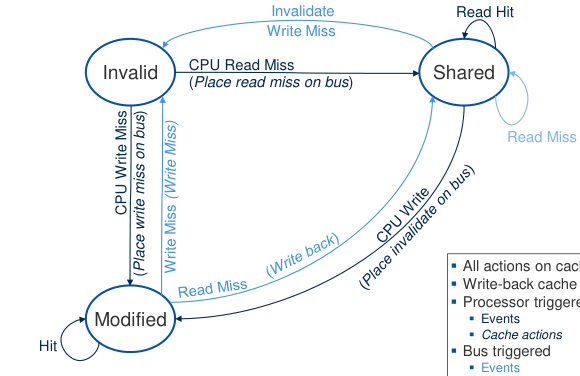
\includegraphics[width=0.8\linewidth]{img/MSIDiagram.png}
  \label{fig:msidiagram}
\end{center}

\begin{center}
  \centering
  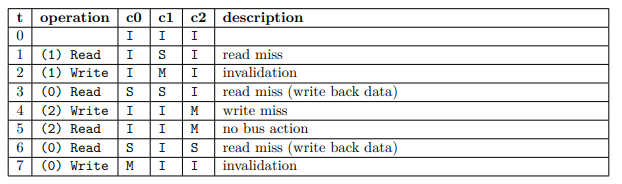
\includegraphics[width=0.8\linewidth]{img/msiExercise.png}
  \label{fig:msiexercise}
\end{center}

\paragraph{example coherency protocl (MESI)} additional exclusive state , beneficial if many writes happen to one address (less invalidations)

\begin{center}
  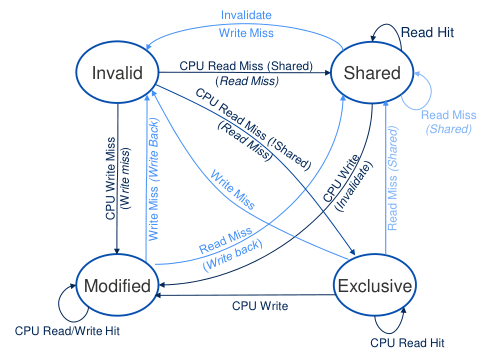
\includegraphics[width=0.8\linewidth]{img/MESIStates.png}
  \label{fig:mesistates}
\end{center}


\begin{center}[h]
  \centering
  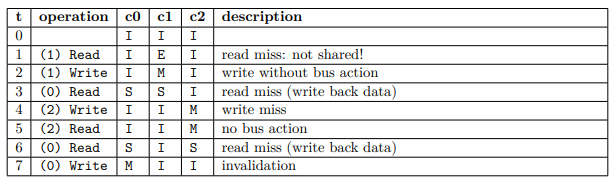
\includegraphics[width=0.8\linewidth]{img/MESIExercise.png}
  \label{fig:mesiexercise}
\end{center}


\paragraph{example coherency protocl (MOSI)} has additional owner state. When there is a read miss and a sharing cache line is in modified state, it goes into owner state that now provides the data instead of writing the data back to memory and providing it from memory. Useful when dram access is really slow.
\begin{center}
  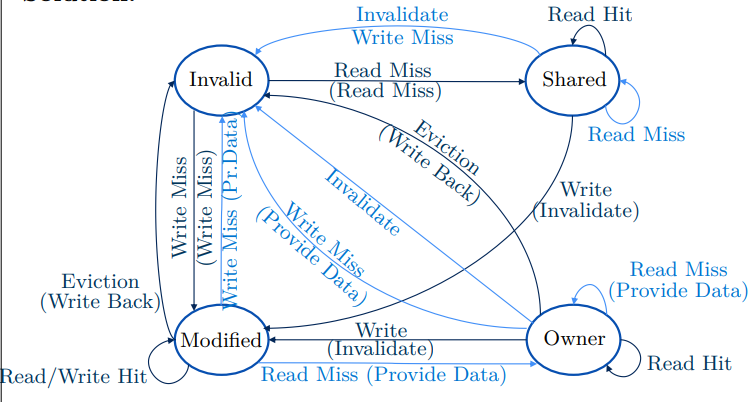
\includegraphics[width=0.8\linewidth]{img/MOSI.png}
  \label{fig:mosi}
\end{center}

\paragraph{Shared Memory without a shared bus} use NoC instead of bus to reduce contentions. Caches do not observe all other acceses.

\paragraph{Why use directory instead of snooping} Snooping is inefficient: Necessity to broadcast all misses and invalidations; Blocking of whole interconnect required for atomicity of actions

\paragraph{Directory-based Cache Coherency}

Sharing status of each block in one location,To increase performance: local copy of own state, Especially for distributed memory, Explicit messages for coherence protocols

\noindent
\coloreq{bits_{directory} = (N_{bits,cacheline} + p) \cdot \frac{cache_{size,shared}}{blocksize_l}}

\coloreq{bits_{directory} = (3bits + p) \cdot \frac{c_2}{blocksize_l}}

\paragraph{Consistency Models}

\begin{enumerate}
  \item[$\bullet$] Sequential Consistency
  \item[$\bullet$] Relaxed Consistency
  \item[$\bullet$] Weak Consistency 
  \item[$\bullet$] Release Consistency
\end{enumerate}

\section{interconnects} oo

\paragraph{Traditional Interconnects: Bus} ..

\paragraph{Traditional Interconnects: Bridged Buses} ..

\paragraph{Traditional Interconnects: Crossbar} 

\begin{center}
  \centering
  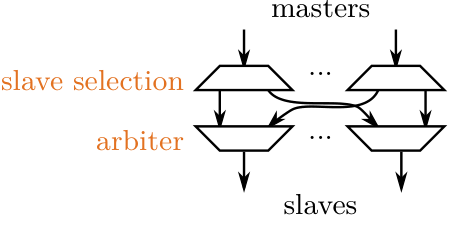
\includegraphics[width=0.4\linewidth]{img/crossbar.png}
  \label{fig:crossbar}
\end{center}

\textbf{Best Case:} all n masters uses n different slaves

\coloreq{BW_{crossbar,bc} = n \cdot BW_{BUS}}

\textbf{Worst Case}: all n masters want to use the same slave

\coloreq{BW_{crossbar,wc} = BW_{BUS}}


\paragraph{Traditional Interconnects: Bi-directional ring} ..

\begin{multicols*}{2}
  Uses less resources than a crossbar but can have higher bandwidth than a bus. It is really good when there is a lot of neighboring traffic. It has an increased latency for long distances
\begin{center}
  \centering
  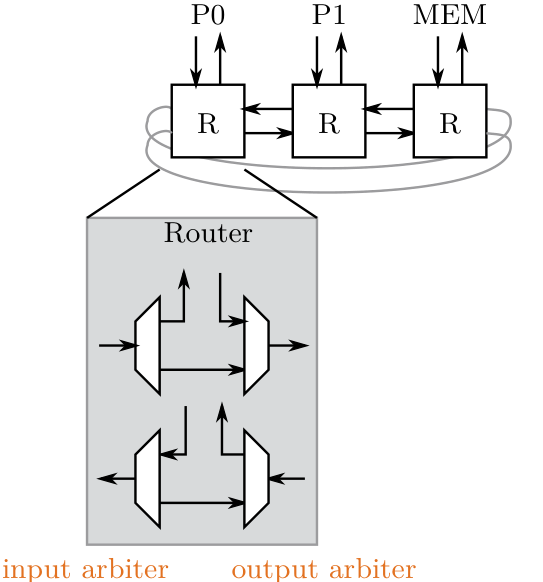
\includegraphics[width=0.8\linewidth]{img/bi-directional ring.png}
  \label{fig:bi-directional-ring}
\end{center}
\end{multicols*}

\paragraph{Network-on-Chip Paradigm} ..

\paragraph{Regular Tiled Structure}..

\paragraph{NoC Building Blocks: Router and Links}..

\paragraph{Network-on-Chip: Segmentation of Wires}..

\paragraph{NoC Performance Metrics}..

\paragraph{Performance of NoCs}..

\paragraph{Topologies}..

\begin{center}
  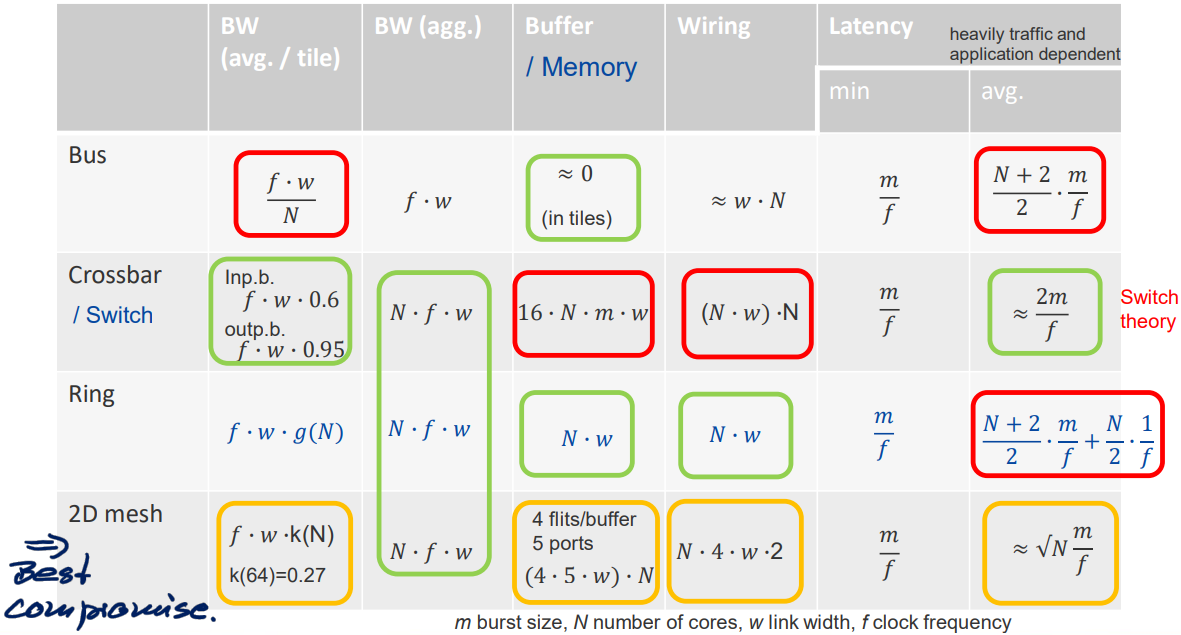
\includegraphics[width=\linewidth]{img/interconnect_summary.png}
  \label{fig:interconnect_summary}
\end{center}

\paragraph{Regular Topoloiges}..

\paragraph{Hierarchical Multi-Topology NoCs}..

\paragraph{Data Units in Networks-on-Chip}..

\paragraph{Forwarding Schemes} Determines how data units travel through the network

\paragraph{Store and Forward} A packet has to be completely received by a router, before it starts to send the packet to the next router.

\coloreq{MinLatency = \frac{PL}{BW} \cdot H(x, y)}

\coloreq{MaxPacketRate = \frac{BW}{PL}}

\paragraph{Wormhole Forwarding} Bits are partitioned into flits(flow control unit). A \textbf{flit} is the smallest unit on which flow control is applied.

+ small buffers (2-4 flits), low latency

\coloreq{Min.Latency = \frac{FL}{BW} \cdot H(x,y) + \frac{PL - FL}{BW}}

where FL: flit length, Pl: Packet length, BW link bandwidth

\coloreq{Max.packetRate = \frac{BW}{PL}}

\paragraph{Comparison of SAF and Wormhole Forwarding}

\begin{center}
  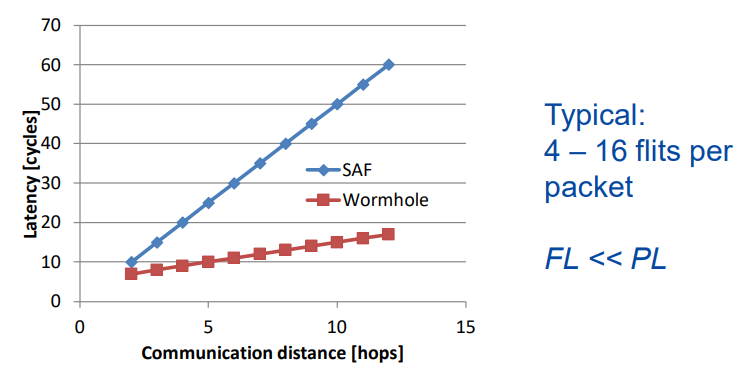
\includegraphics[width=0.8\linewidth]{img/cmpSAFWormhole.png}
  \label{fig:cmpsafwormhole}
\end{center}

\paragraph{Blocking in Wormhole Forwarding}..

\paragraph{Virtual Channels} have their own buffer and routing logic but only one virtual channel can recieve/send at a specific cycle.

+ avoid deadlocks, reduces the impact of contentions on latency

- additional hw resources

\textbf{contention:} two input ports trying to access the same output port


\begin{center}
  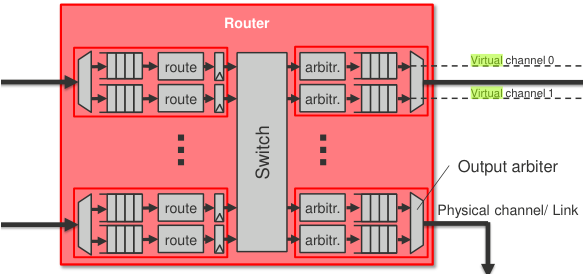
\includegraphics[width=0.8\linewidth]{img/virtual_channel.png}
  \label{fig:virtual_channel}
\end{center}

\paragraph{Bufferless Forwarding}
Bufferless forwarding inefficient: 
\begin{enumerate}
  \item[$\bullet$] Every contention leads to drop high drop rate, wastes bandwidth by retransmission
  \item[$\bullet$] Misrouting wastes bandwidth by sending packets in wrong directions
\end{enumerate}

\paragraph{Routing Algorithms}..

\paragraph{Deadlocks}
Routing dependent deadlock: caused by improper routing in the NoC

Message dependent deadlocks
\paragraph{Channel Dependency Diagram}..

\begin{center}
  \centering
  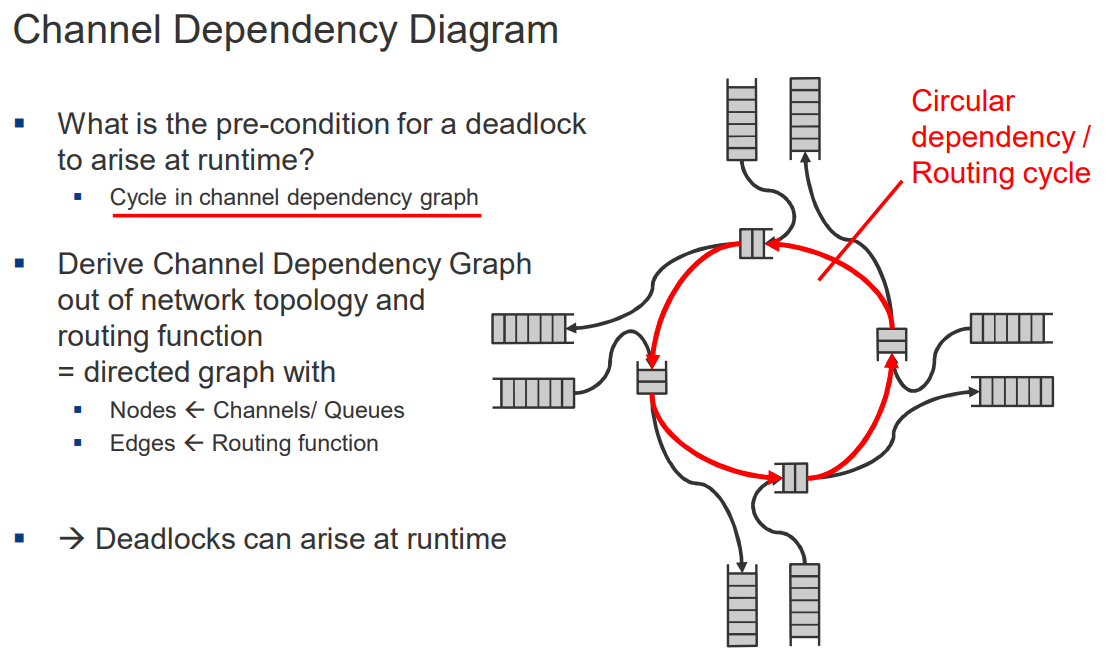
\includegraphics[width=0.8\linewidth]{img/ChanelDependencyDiagram.png}
  \label{fig:chaneldependencydiagram}
\end{center}

\paragraph{Tackling Deadlocks} \mbox{}

deadlock avoidance vs deadlock recovery

\paragraph{Deadlock Avoidance} \mbox{}

\textbf{Uni-directional} ring NoC - 2 virtual channels, route in spiral fashion - requests to VC1, response to VC2

\textbf{XY-Routing} prohibits turns from y to x direction, only x-x and y-y, 2 turns per cycle not allowed, nod-adaptive/deterministic, deadlock free, minimal


\begin{center}
  \centering
  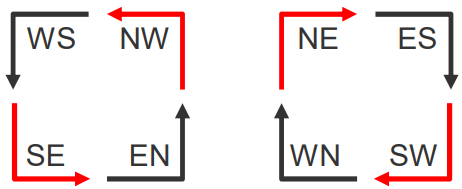
\includegraphics[width=0.4\linewidth]{img/xy_routing.png}
  \label{fig:xy_routing}
\end{center}

\textbf{Turn Model} (adaptive routing possible) 

\textit{West First:} prohibits turns to west: NW and SW, packets destined to west have to start in west direction (no turn to west later), 1 turn per cycle is not allowed adaptive(multiple paths exist) deadlock free

\begin{center}
  \centering
  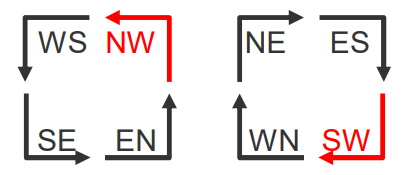
\includegraphics[width=0.4\linewidth]{img/west_first.png}
  \label{fig:west_first}
\end{center}

\textit{North last:} (prohibits NW and NE), etc.


\paragraph{Adaptive Routing}\mbox{}

Select a path from x to y out of all paths $R_{xy}$ considering the state of the network

- Livelocks can occur if non-minimal paths are allowed!

\paragraph{Protocols \& Message Dependencies}..

\paragraph{Message Dependent Deadlocks}..

\section{Operating Systems} \textcolor{red}{not required for exam}

Interface between application software  and 
hardware resources (processor with instruction 
set architecture ISA, devices, memory)

memory management

Access of I/O devices, network, file system

Inter Process Communication (IPC)

Interrupt handling

\paragraph{Classification}

Single/Multitasking, Single/Multiple users, Single/Multithread, Single/Multiprocessor, RTOS

\paragraph{Processes}Instance of application program being executed

\section{exam questions} \mbox{} \\
\textit{You have a SoC in which two CPU core are connected to two memories over a mesh [3] NoC. The NoC uses XY routing. CPU 1 sends requests to memory 1, CPU 2 sends requests to memory 2. How many virtual channels do you use in your NoC? Explain your answer.}

at least two, to avoid message-dependent deadlocks

• message-dependent deadlocks are separate from routing-dependent deadlocks

\textit{For East Last routing: clearly mark the forbidden turns in the turn model below and complete the Channel Dependency Diagram for a 2 × 2 mesh network.}

\begin{center}
  \centering
  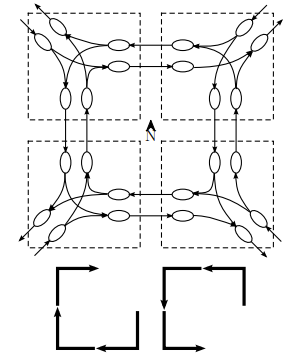
\includegraphics[width=0.8\linewidth]{img/east last routing.png}
  \label{fig:east-last-routing}
\end{center}

\textit{Discuss the benefits and drawbacks of heterogeneous multi-core systems, comparedto homogeneous multi-core systems. Support your argumentation with a qualitativegraph.}

benefit: higher computational density of hw accelerators•drawback: higher programming effort, use of more area, higher design com-plexity•graph: computational density (for example, others are possible as well)

\textit{In your words explain why Peterson Lock can only work for two threads}

Solution: This lock uses a variable called victim and each thread that sets thisvariable latest has to wait for the other thread to enter the critical section. If morethan 2 threads are used we need more than just one victim variable, because morethan one thread will then think they are not the victim and hence may access theshared data.

\textit{What is the basic idea behind Transactional Memory in the context of synchroniza-tion?}

The central argument behind TM is that synchronization and consis-tency of all data should actually not be the problem of the programmer. Insteadthe programmer should just define a block of instructions as atomic. Inside thisblock any data should be modified and even function calls are allowed.

\textit{Why is it necessary to always lock both the predecessor and the element to bedeleted?}

Solution: Because it must be ensured that between the predecessor and thenode to be deleted nothing is inserted in the data structure

\textit{Perform the below given operation using the MSI protocol. Use the cache state asshown in the figure above.Draw a message sequence chart with the messages exchanged between the caches andthe directory. Make sure to label the messages.Which index of the processor has changed and what is the changed state of that index?}

\begin{center}
  \centering
  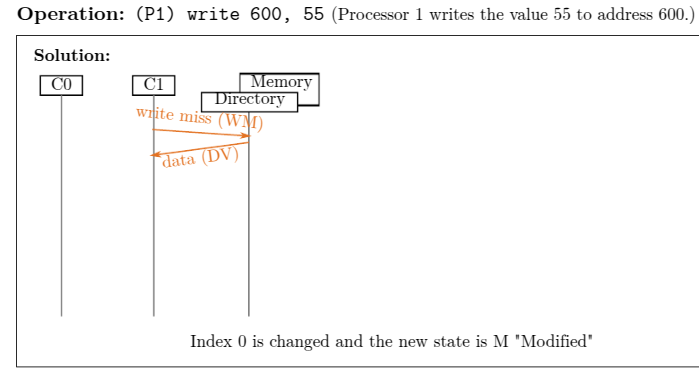
\includegraphics[width=0.8\linewidth]{img/mseqchart.png}
  \label{fig:mseqchart}
\end{center}

\textit{Explain the shift in System-on-Chip design to multi-core architectures. What meth- [8]
ods to improve performance were used before (name at least two examples)? Why were
different approaches needed? Support your argumentation with a qualitative graph.}

no more pure voltage/frequency scaling
• microarchitecture improvements (exampes: pipeline depth, multi-isuse pipelines,
improved branch prediction) have become less efficient regarding power and
area (measured in dIPC/dPower and dIPC/dArea)
• => shift to macro-architecture improvements necessary
• graph: usually moore’s law (power wall)




\end{multicols*}

\end{document}
